\appendix

\chapter{\label{appendixa}Grid description examples}

\section{Example of a curvilinear grid description}
Here is an example for the \CDO description of a curvilinear grid.
xvals/yvals describes the position of the 6x5 quadrilateral grid cells.
The first 4 values of xbounds/ybounds are the corners of the first grid cell.
\begin{lstlisting}[frame=single, backgroundcolor=\color{zebg}, basicstyle=\footnotesize]
gridtype  : curvilinear
gridsize  : 30
xsize     : 6
ysize     : 5
xvals     :  -21  -11    0   11   21   30  -25  -13    0   13
              25   36  -31  -16    0   16   31   43  -38  -21
               0   21   38   52  -51  -30    0   30   51   64
xbounds   :  -23  -14  -17  -28       -14   -5   -6  -17        -5    5    6   -6
               5   14   17    6        14   23   28   17        23   32   38   28
             -28  -17  -21  -34       -17   -6   -7  -21        -6    6    7   -7
               6   17   21    7        17   28   34   21        28   38   44   34
             -34  -21  -27  -41       -21   -7   -9  -27        -7    7    9   -9
               7   21   27    9        21   34   41   27        34   44   52   41
             -41  -27  -35  -51       -27   -9  -13  -35        -9    9   13  -13
               9   27   35   13        27   41   51   35        41   52   63   51
             -51  -35  -51  -67       -35  -13  -21  -51       -13   13   21  -21
              13   35   51   21        35   51   67   51        51   63   77   67
yvals     :   29   32   32   32   29   26   39   42   42   42
              39   35   48   51   52   51   48   43   57   61
              62   61   57   51   65   70   72   70   65   58
ybounds   :   23   26   36   32        26   27   37   36        27   27   37   37
              27   26   36   37        26   23   32   36        23   19   28   32
              32   36   45   41        36   37   47   45        37   37   47   47
              37   36   45   47        36   32   41   45        32   28   36   41
              41   45   55   50        45   47   57   55        47   47   57   57
              47   45   55   57        45   41   50   55        41   36   44   50
              50   55   64   58        55   57   67   64        57   57   67   67
              57   55   64   67        55   50   58   64        50   44   51   58
              58   64   72   64        64   67   77   72        67   67   77   77
              67   64   72   77        64   58   64   72        58   51   56   64
\end{lstlisting}

\begin{figure}[b]
{\scalebox{0.99}{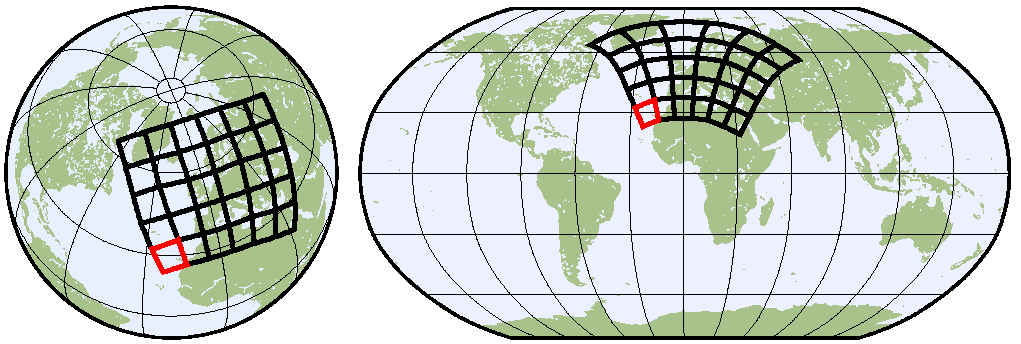
\includegraphics{grids/curv.pdf}}}
\caption[curvgrid]{Orthographic and Robinson projection of the curvilinear grid}
\end{figure}

\newpage
\section{Example description for unstructured grid cells}
Here is an example of the \CDO description for unstructured grid cells.
xvals/yvals describes the position of 30 independent hexagonal grid cells.
The first 6 values of xbounds/ybounds are the corners of the first grid cell.
\begin{lstlisting}[frame=single, backgroundcolor=\color{zebg}, basicstyle=\footnotesize]
gridtype  : cell
gridsize  : 30
nvertex   : 6
xvals     :  -36   36    0  -18   18  108   72   54   90  180 
             144  126  162 -108 -144 -162 -126  -72  -90  -54
               0   72   36  144  108 -144  180  -72 -108  -36 
xbounds   :  339    0    0  288  288  309        21   51   72   72    0    0
               0   16   21    0  339  344       340    0   -0  344  324  324
              20   36   36   16    0    0        93  123  144  144   72   72
              72   88   93   72   51   56        52   72   72   56   36   36
              92  108  108   88   72   72       165  195  216  216  144  144
             144  160  165  144  123  128       124  144  144  128  108  108
             164  180  180  160  144  144       237  267  288  288  216  216
             216  232  237  216  195  200       196  216  216  200  180  180
             236  252  252  232  216  216       288  304  309  288  267  272
             268  288  288  272  252  252       308  324  324  304  288  288
             345  324  324   36   36   15        36   36  108  108   87   57
              20   15   36   57   52   36       108  108  180  180  159  129
              92   87  108  129  124  108       180  180  252  252  231  201
             164  159  180  201  196  180       252  252  324  324  303  273
             236  231  252  273  268  252       308  303  324  345  340  324
yvals     :   58   58   32    0    0   58   32    0    0   58
              32    0    0   58   32    0    0   32    0    0
             -58  -58  -32  -58  -32  -58  -32  -58  -32  -32 
ybounds   :   41   53   71   71   53   41        41   41   53   71   71   53
              11   19   41   53   41   19       -19   -7   11   19    7  -11
             -19  -11    7   19   11   -7        41   41   53   71   71   53
              11   19   41   53   41   19       -19   -7   11   19    7  -11
             -19  -11    7   19   11   -7        41   41   53   71   71   53
              11   19   41   53   41   19       -19   -7   11   19    7  -11
             -19  -11    7   19   11   -7        41   41   53   71   71   53
              11   19   41   53   41   19       -19   -7   11   19    7  -11
             -19  -11    7   19   11   -7        11   19   41   53   41   19
             -19   -7   11   19    7  -11       -19  -11    7   19   11   -7
             -41  -53  -71  -71  -53  -41       -53  -71  -71  -53  -41  -41
             -19  -41  -53  -41  -19  -11       -53  -71  -71  -53  -41  -41
             -19  -41  -53  -41  -19  -11       -53  -71  -71  -53  -41  -41
             -19  -41  -53  -41  -19  -11       -53  -71  -71  -53  -41  -41
             -19  -41  -53  -41  -19  -11       -19  -41  -53  -41  -19  -11
\end{lstlisting}

\begin{figure}[b]
{\scalebox{1}{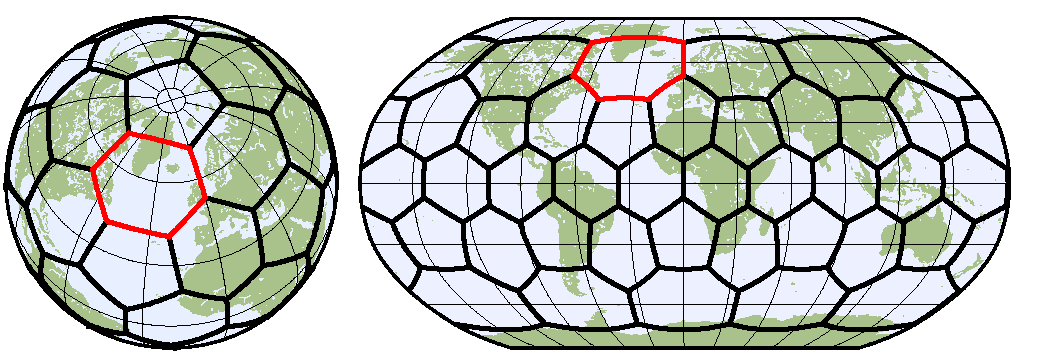
\includegraphics{grids/cell.pdf}}}
\caption[cellgrid]{Orthographic and Robinson projection of the unstructured grid cells}
\end{figure}

%%% Local Variables: 
%%% mode: latex
%%% TeX-master: "grid"
%%% End: 
